\documentclass{article}
\usepackage[a4paper, margin=2.5cm]{geometry}
\usepackage[utf8]{inputenc}
\usepackage{amsmath}
\usepackage{amssymb}
\usepackage{derivative}
\usepackage[most]{tcolorbox}
\tcbuselibrary{listingsutf8}
\usepackage{graphicx}
\usepackage{float}

\tcbset{
  promptbox/.style={
    enhanced,
    colback=blue!5,
    colframe=blue!60!black,
    boxrule=0.8pt,
    arc=3mm,
    left=6pt,
    right=6pt,
    top=6pt,
    bottom=6pt,
    fonttitle=\bfseries,
    title=Prompt,
  }
}

% Style listings pour Python
\lstdefinestyle{mypython}{
    language=Python,
    backgroundcolor=\color{gray!10},
    basicstyle=\ttfamily\small,
    keywordstyle=\color{blue}\bfseries,
    stringstyle=\color{orange},
    commentstyle=\color{green!50!black},
    numbers=left,
    numberstyle=\tiny,
    stepnumber=1,
    frame=none
}

% Boîte pour code Python
\newtcblisting{pythonbox}{
  listing only,
  listing options={style=mypython},
  colback=gray!10,
  colframe=blue!50!black,
  boxrule=0.5pt,
  arc=3mm,
  left=5pt,
  right=5pt,
  top=5pt,
  bottom=5pt
}

\title{Projet 1 : MS01}
\author{Clément Baillet et Paul Michel}
\date{}

\begin{document}
\maketitle

\section{Méthode de Jacobi}
Dans toute la suite du rapport, les exemples sont réalisés pour les données suivantes : $U_0 = 1$, $\Omega = \,]0, 1[ \times \,]0, 1[$, $\alpha = 0,5$ ; et on fixe une tolérance en précision de $10^{-6}$ ainsi qu'un nombre maximal d'itérations à $10 000$ sauf mention contraire. \\
Pour un nombre de points intérieurs $N = 50$ (selon $x$ et selon $y$), on converge après $4235$ itérations avec une erreur finale légèrement inférieure à $10^{-6}$ :

\begin{figure}[H]
    \centering
    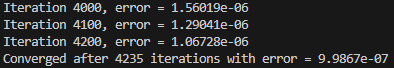
\includegraphics[width=0.9\textwidth]{test_jacobi_seq.png}
    \caption{Exemple d'exécution du code séquentiel - méthode de Jacobi}
    \label{fig:Jacseq}
\end{figure}

En effectuant des tests  pour $N_x \in [50,100,150,200,250]$, on observe une tendance $n_{iter} \propto N_x^{1,35}$. Le fait que l'on trouve 1,35 plutôt que 2 est peut-être dû au fait que garder $Ny=50$ réduise la dépendance pure $Nx^2$; cela est éventuellement influencé par le critère d'arrêt pour des petites grilles comme celles étudiées.

\begin{figure}[H]
    \centering
    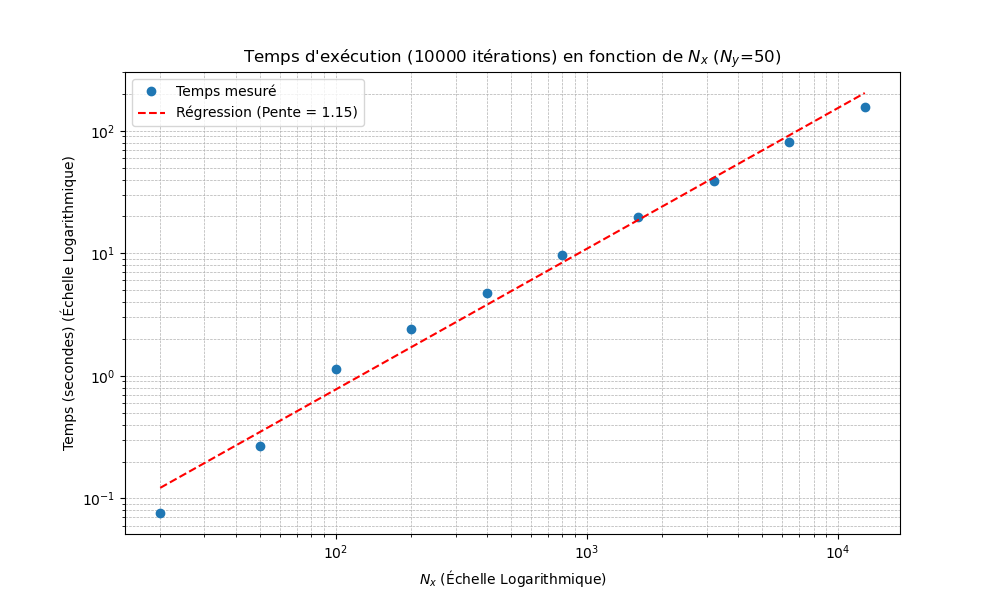
\includegraphics[width=0.9\textwidth]{courbe_log_log_jacobi.png}
    \caption{Evolution du nombre d'itérations en fonction de Nx - méthode de Jacobi}
    \label{fig:loglogJac}
\end{figure}

\section{Méthode de Gauss-Seidel}
Pour le même jeu de données, on converge plus rapidement grâce à la technique de Gauss-Seidel :

\begin{figure}[H]
    \centering
    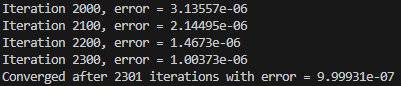
\includegraphics[width=0.9\textwidth]{test_gaussseidel_seq.png}
    \caption{Exemple d'exécution du code séquentiel - méthode de Gauss-Seidel}
    \label{fig:GSseq}
\end{figure}

De même que pour Jacobi, en effectuant des tests  pour $N_x \in [50,100,150,200,250]$, on observe une tendance $n_{iter} \propto N_x^{1,37}$. A nouveau, il est possible que la loi asymptotique s'observe mieux avec davantage de tests pour des $N_x$ plus élevés.

\begin{figure}[H]
    \centering
    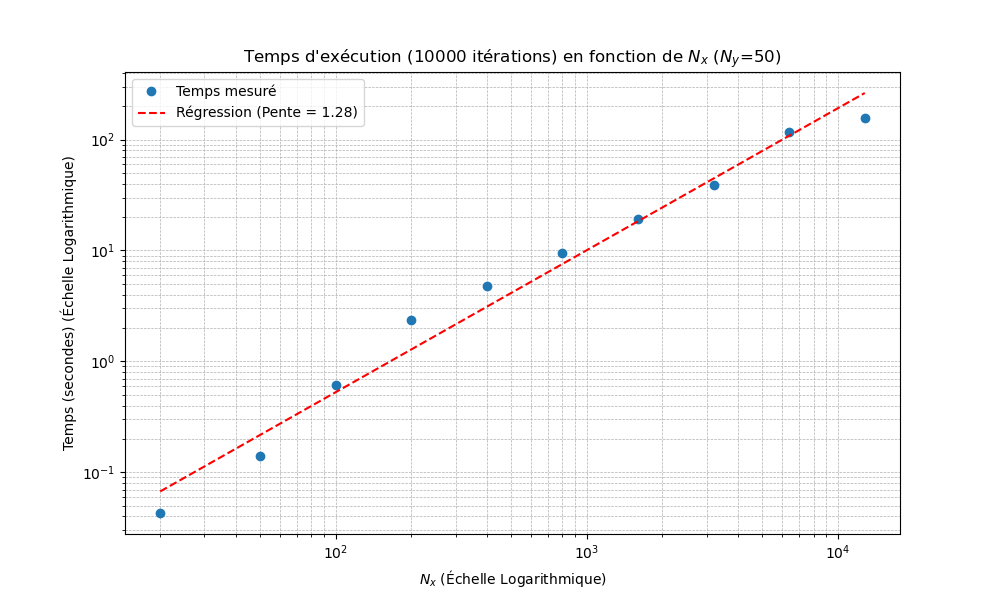
\includegraphics[width=0.9\textwidth]{courbe_log_log_gs.png}
    \caption{Evolution du nombre d'itérations en fonction de Nx - méthode de Gauss-Seidel}
    \label{fig:loglogGS}
\end{figure}

\section{Comparaison des deux approches}
Dans la méthode de Jacobi, on met à jour $u$ à la fin de chaque boucle, alors que pour Gauss-Seidel on le fait dans la boucle même. Cela implique l'utilisation de 2 tableaux représentant $u$ pour Jacobi, alors qu'un seul suffit pour Gauss-Seidel.\\
Cette observation sur le plan logique des méthodes est confirmée par la différence du nombre d'itérations avant convergence : Gauss-Seidel est une méthode presque deux fois plus rapide que celle de Jacobi en ce sens d'après les figures $1$ et $2$. \\
Plus encore, en comparant le temps d'exécution entre les deux approches, on remarque une fois de plus que celle de Gauss-Seidel est plus rapide.

La comparaison des deux précédentes parties sur l'évolution du nombre d'itérations en fonction de la taille de la grille se visualise par la figure qui suit:

\begin{figure}[H]
    \centering
    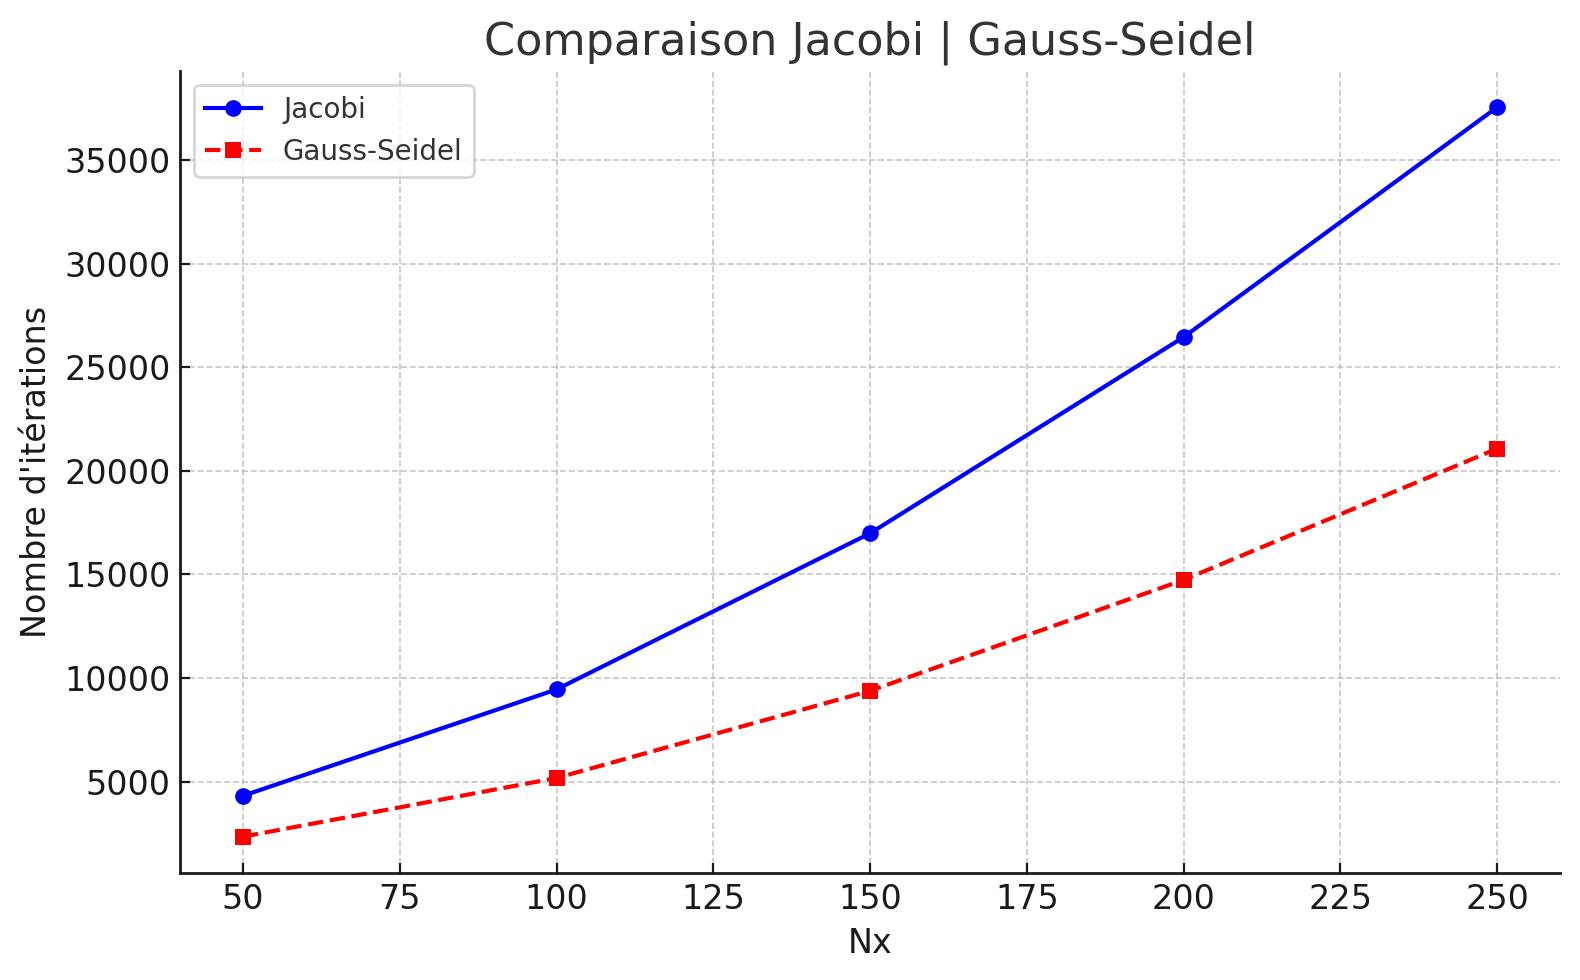
\includegraphics[width=0.9\textwidth]{comparaison_j_gs.png}
    \caption{Comparaison de l'évolution du nombre d'itérations en fonction de Nx}
    \label{fig:comparaison}
\end{figure}

\section{Parallélisation du code : Jacobi}

Dans cette sous-section uniquement, les tests ont été réalisés sur une grille 500x500 avec 1 jusqu'à 6 processeurs sur une machine de l'ENSTA. Le graphe ci-dessous permet l'étude de la scalabilité forte de la méthode de Jacobi:


\begin{figure}[H]
    \centering
    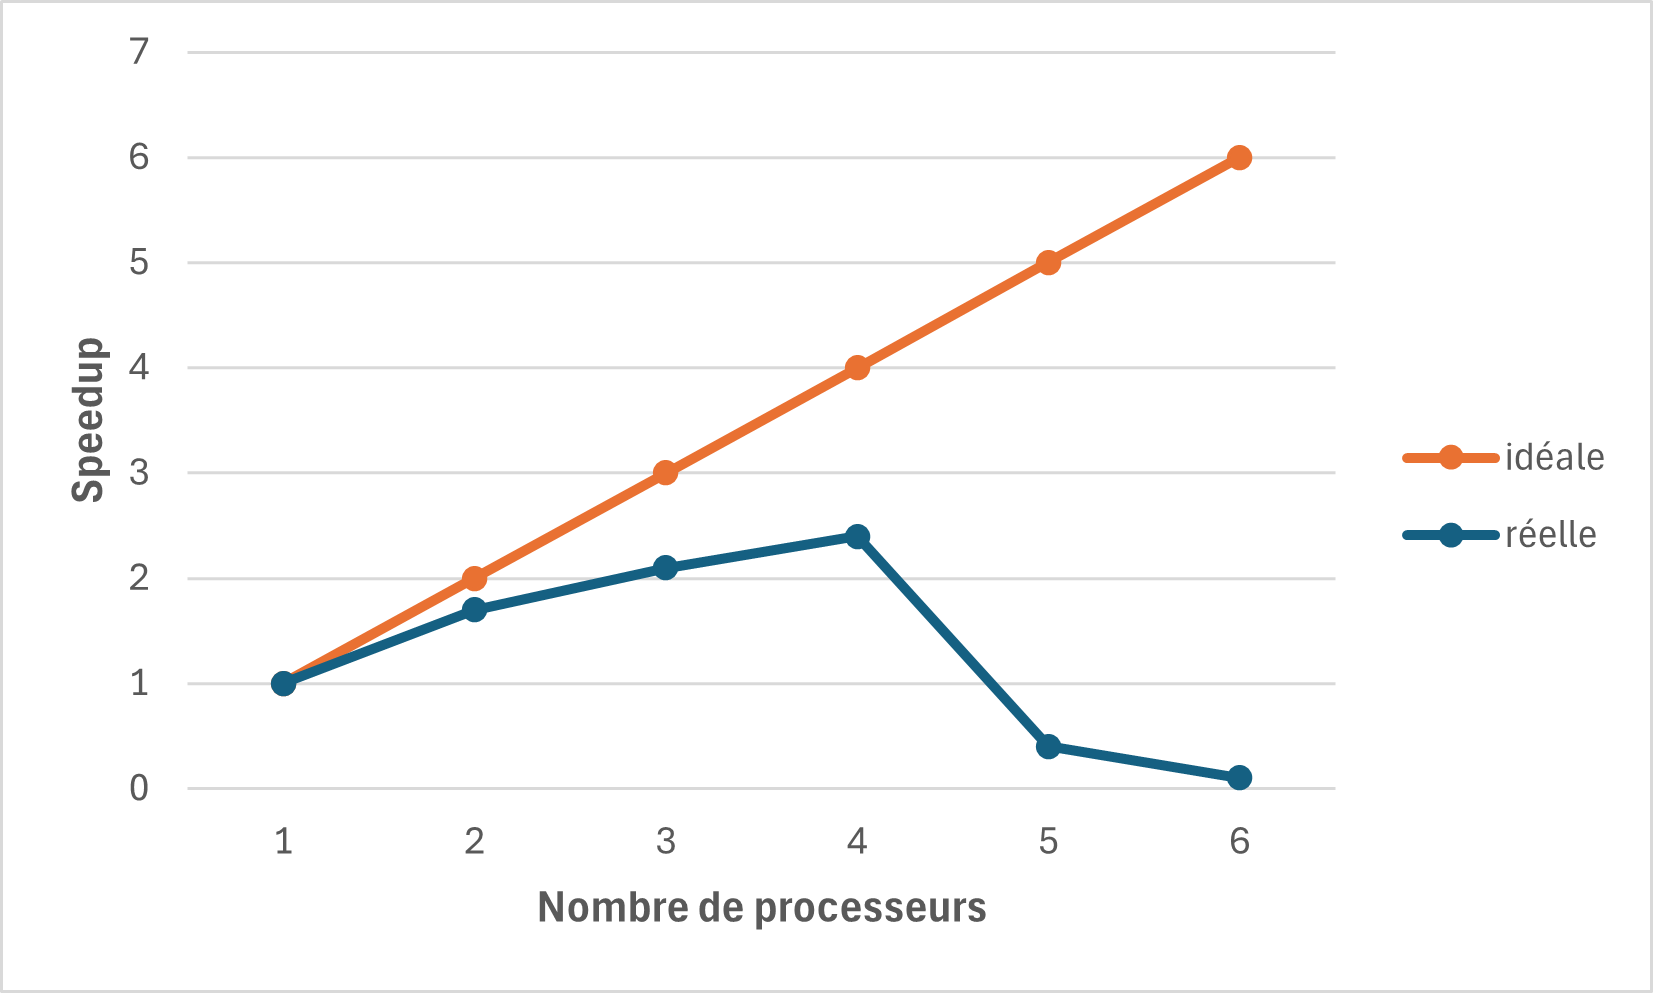
\includegraphics[width=0.9\textwidth]{strong_scaling_jacobi.png}
    \caption{Scalabilité forte - méthode de Jacobi}
    \label{fig:strongJac}
\end{figure}

On observe que le speedup croît avec le nombre de processeurs tant qu'on se sert de moins de 4 coeurs, limite après laquelle le speedup s'effondre. Sur la partie croissante, on observe une bonne scalabilité forte pour la méthode de Jacobi.

On peut constater ces mêmes résultats en étudiant l'évolution de l'efficiency en fonction du nombre de processeurs grâce au graphique suivant :

\begin{figure}[H]
    \centering
    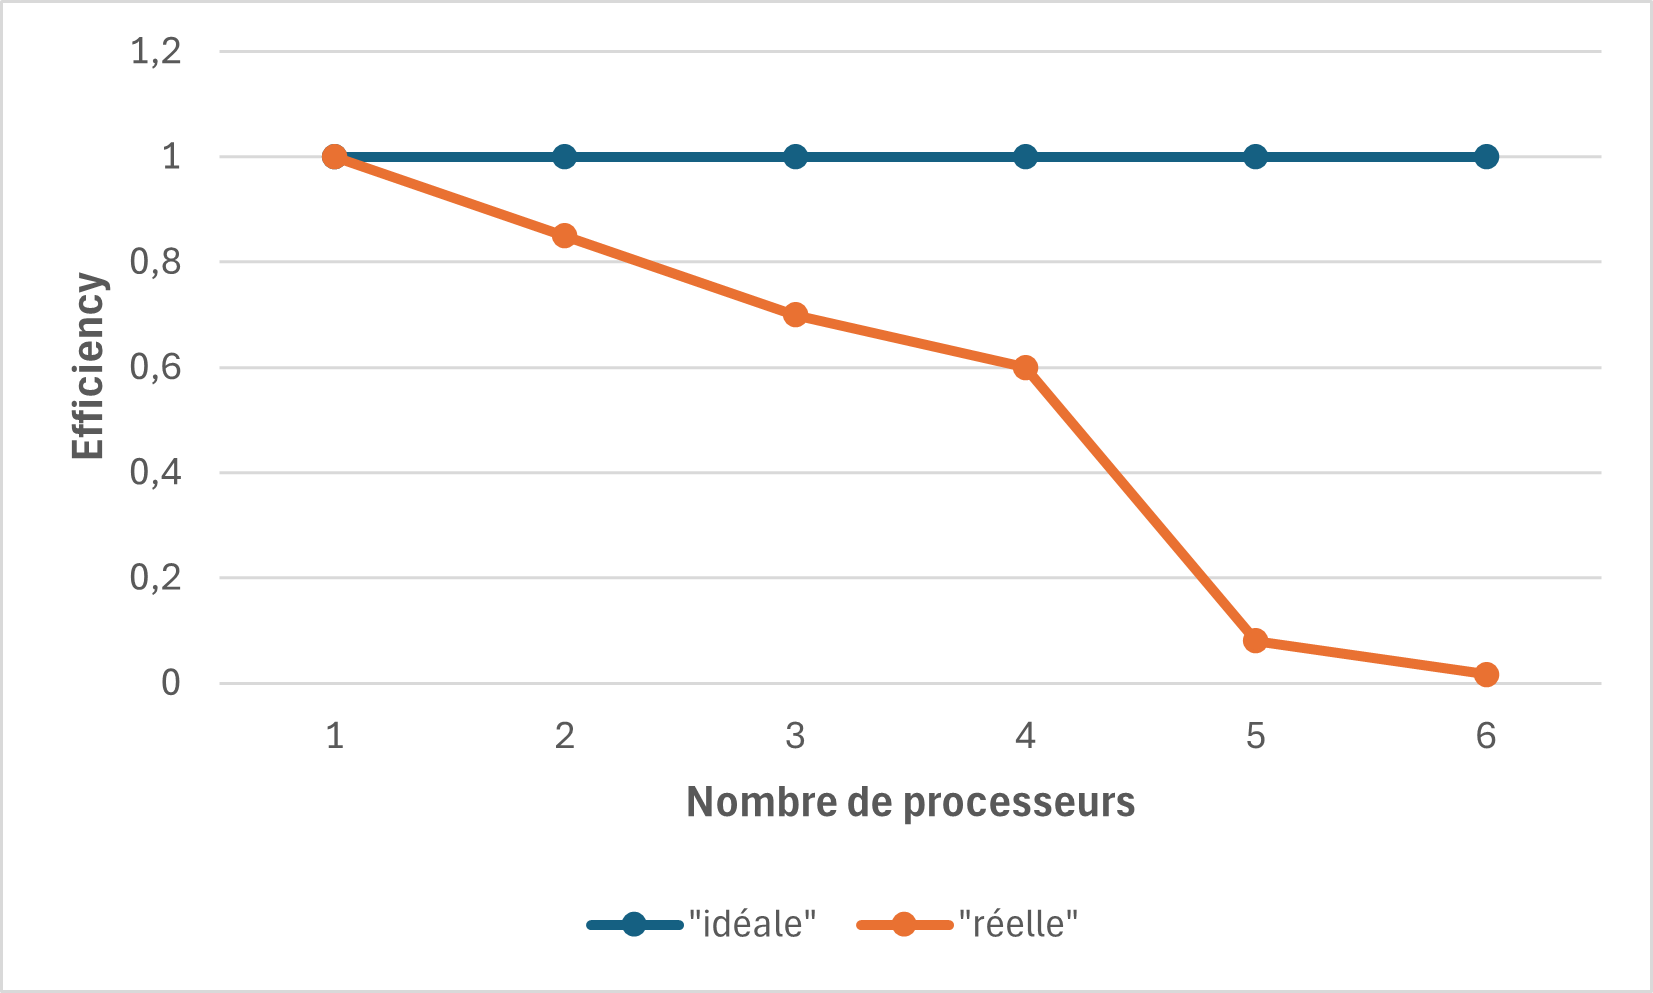
\includegraphics[width=0.9\textwidth]{weak_scaling_jacobi.png}
    \caption{Scalabilité faible - méthode de Jacobi}
    \label{fig:weakJac}
\end{figure}

Il est intéressant de remarquer qu'après avoir effectué des tests sur différentes tailles de grilles, on constate pour un petit format (50x50) un scaling moindre que pour des plus grandes grilles (300x300). Cela semble cohérent car une plus grande taille rend la parallélisation davantage intéressante.


\section{Parallélisation du code : Gauss-Seidel}

Bien que les différents tests ont montré que généralement Gauss-Seidel convergeait en moins d'itérations que Jacobi (idéalement 2x moins), la scalabilité forte de cette méthode est moins bonne que celle de Jacobi, notamment à cause d'un plus grand nombre de communications avec la méthode Rouge/Noir. Le graphique suivant montre les résultats obtenus pour la méthode de Gauss-Seidel et compare avec la scalabilité forte de Jacobi :

\begin{figure}[H]
    \centering
    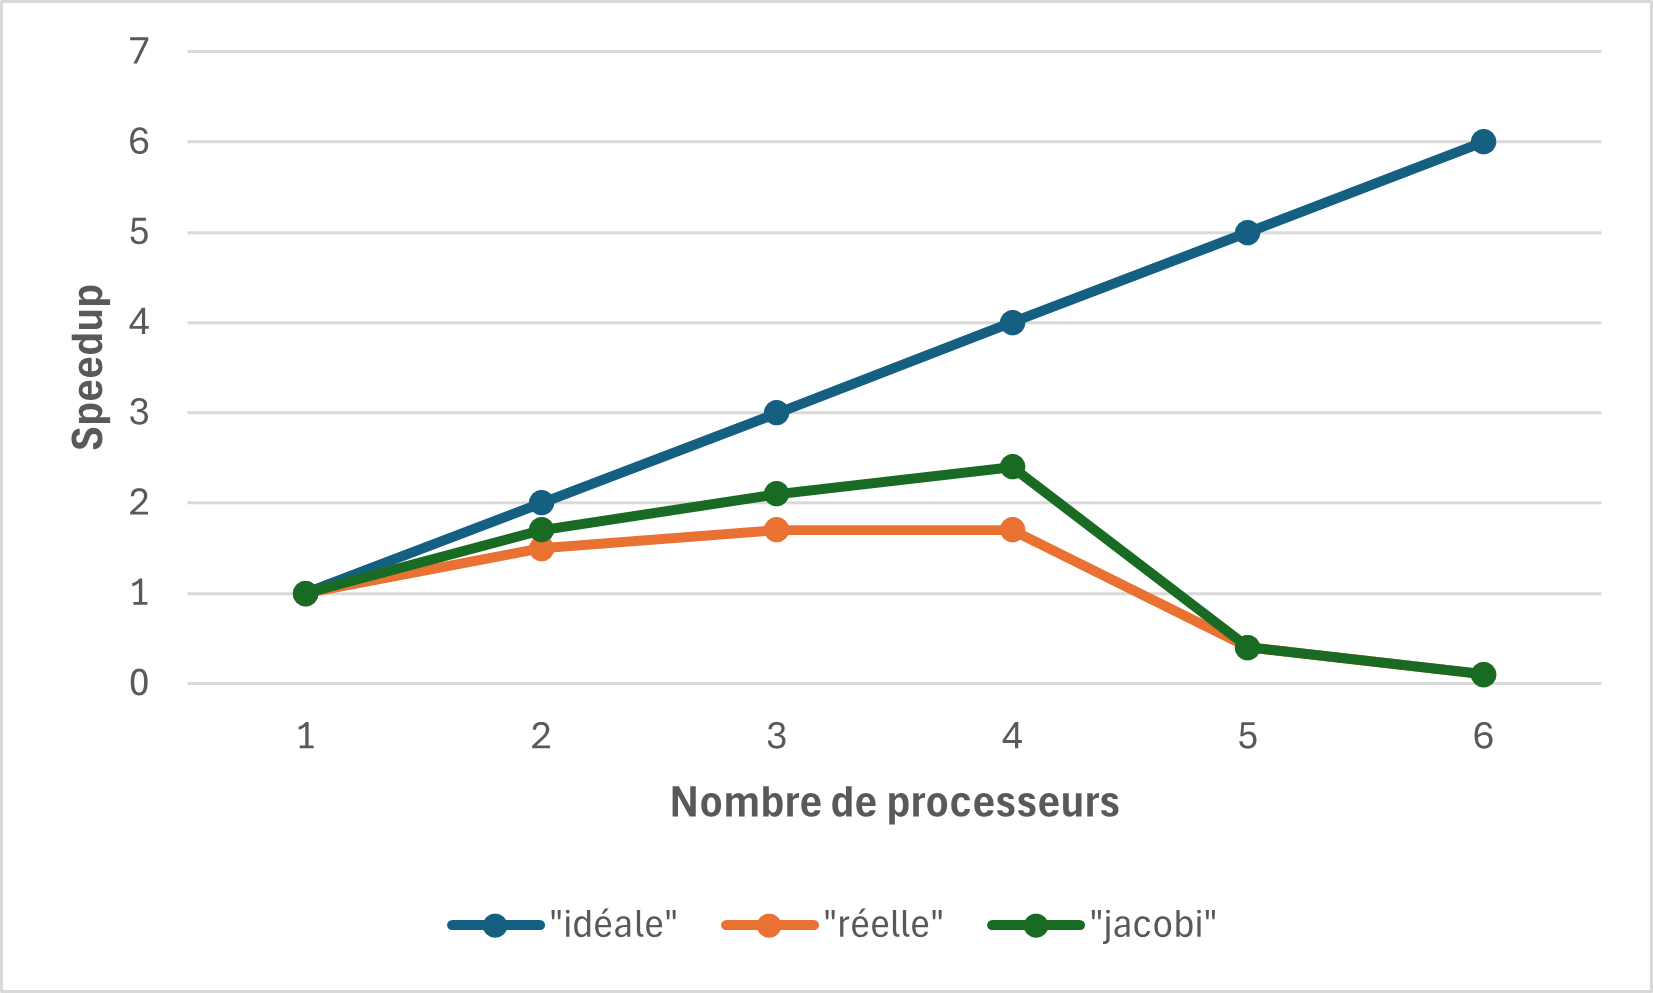
\includegraphics[width=0.9\textwidth]{strong_scaling_gs.png}
    \caption{Scalabilité forte - Gauss-Seidel et comparaison}
    \label{fig:strongGS}
\end{figure}

\section{Tests avec Cholesky}

\begin{figure}[H]
    \centering
    \includegraphics[width=0.9\textwidth]{Scalabilité_Forte_Speedup}
    \caption{Scalabilité faible - Cholesky}
    \label{fig:strongCholesky}
\end{figure}

\begin{figure}[H]
    \centering
    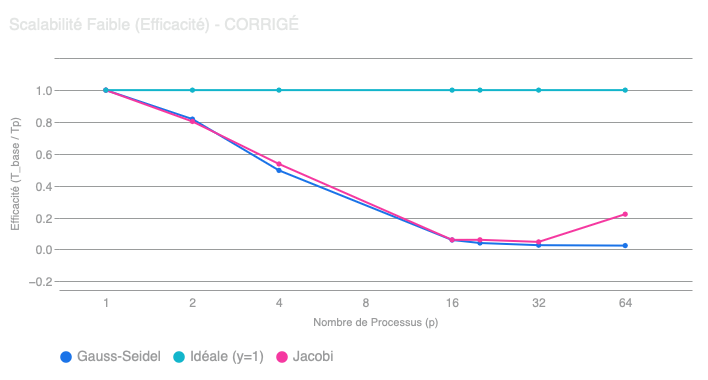
\includegraphics[width=0.9\textwidth]{Scalabilité_Faible_Efficacité}
    \caption{Scalabilité faible - Cholesky}
    \label{fig:weakCholesky}
\end{figure}

Pour les tests sur le mésocentre Cholesky, comme pour la méthode Jacobi, nous avons testé la scalabilité forte pour une tolérance de $10^{-8}$, et sur un domaine fixe de $256\times 256$. Pour la scalabilité faible, nous avons augmenté progressivement la taille du domaine, en passant de $16\times 256$ à $512\times 256$. Les Figures \ref{fig:strongCholesky} et \ref{fig:weakCholesky} montrent les deux scalabilités avec les données obtenus.

Pour le speedup, on observe bien une augmentation quasi linéaire en fonction du nombre de processus, et qui se rapproche de plus en plus du speedup idéal à mesure que la taille du domaine augmente. Idem pour l'efficacité, on voit qu'elle se rapproche de plus en plus de $1$ quand la taille augmente linéairement avec le nombre de processus.

\end{document}